This study evaluated the performance of AcPSVRG for solving logistic regression problem. Here, $f_i(\textbf{w})$ = log(1+$e^{-y_ix^T_i\textbf{w}})+\frac{\lambda}{2}\|\textbf{w}\|^2$, where $\lambda$ is the regularziation hyper-parameter and $(\textbf{x}_i, y_i)$ is the training instance $i$ with feature vector $\textbf{x}_i\in\R^d $ and class label $y_i\in$\{-1, +1\}. 

\subsection{Experiment Setup}
\subsubsection{Datasets}
Three representative datasets are selected from LIBSVM, including covtype, w8a, and ijcnn, which are commonly used for the research on machine learning algorithm or platform performance. The primary metadata of these datasets are summarized in Table \ref{metadata}. Data normalization is completed on each dataset before training.  

\subsubsection{Distributed Platform and Parameter Setting}
Two sets of experiments are developed to accurately assess the performance of AcPSVRG on distributed platform. One is scalability analysis with the comparison between Sync-AcPSVRG and Async-AcPSVRG. The aim of this experiment is to explore the potential speedup of AcPSVRG. The other is to compare AcPSVRG with state-of-the-art variance reduction algorithms, i.e., SVRG, SAGA, and Katyusha, using the same asynchronous platform. For each algorithm, we tried several sets of parameters and selected the one with best performance. All projects were developed using OpenMPI and C++ and performed by use of multiple Amazon EC2 t2.micro instances. The codes will be published when the article is accepted. 

\subsection{Scalability Analysis}
The same parameter server architecture was applied to compare Sync-AcPSVRG and Async-AcPSVRG for scalability analysis. The algorithms were run by one server with different numbers of workers. Iteration and time speedup are calculated by following formula and the results are shown by Figure \ref{fig:FSVRG_speedup}. Both algorithms yield good speedup. In particular, iteration speedup is significantly better than time speedup by virtue of stable convergence of AcPSVRG on distributed platform. Concerning time speedup, Async-AcPSVRG exhibits higher scalability than Sync-AcPSVRG since Async-AcPSVRG saves more synchronization overhead. This result also implies that AcPSVRG exhibits better asynchronous property on parameter server architecture and higher potential for further acceleration with optimized distributed platform.

\subsection{Comparison of Convergence}
The experiments with asynchronous setting were carried out with L2-norm ($\lambda = 10^{-4}$) regularized logistic regression problems and performance of different methods is collated by Figure \ref{fig:algo_comp}. The x-axis indicates effective iterations which are similar to update steps in sequential setting. All of approaches were implemented by parameter server with 1 server and 16 workers. It is obtained that Async-AcPSVRG always exhibits better convergence than any other method. In particular, compared to Katyusha, as a fast momentum acceleration method, AcPSVRG shows significantly better convergence with asynchronous distributed platform. The oscillation of Katyusha results from data partitioning and local worker implements momentum terms with local partial data which introduces variance in training process. In contrast, AcPSVRG, similar to SVRG or ProxASAGA, directs updates relying less on global data, and thus, data partitioning has much less impact on momentum acceleration. This finding further confirmed that AcPSVRG is a superior momentum acceleration method with good asynchronicity.  


\begin{table}
\begin{center}
\caption{Summary of training datasets.}
\begin{tabular}{ c|c|c|c } 
 \hline
 Datasets &  Data & Features & Class  \\ 
 \hline
  covtype & 581,012 & 54 & 2 \\ 
 w8a & 49,749  & 300 & 2 \\ 
 ijcnn & 49,990 & 22 & 2 \\
 %SUSY & 5,000,000 & 18 & 2 \\
 \hline
\end{tabular}
\label{metadata}
\end{center}
\end{table}


\iffalse
\begin{table}
\begin{center}
\caption{Parameter setting for algorithm implementation. Lmax denotes Lipschitz constant, n is the number of data, and $\rho$ and  $m_s$ are specified to 1.25 and n/4. }
\begin{tabular}{ c|c|c|c } 
 \hline
 Algorithms & initial $\eta$ & Inner Loops & $\lambda$  \\ 
 \hline
 SVRG & 1/(10*Lmax) & 2n & 1e-4\\
 SAGA & 1/(10*Lmax) & n & 1e-4\\
 %SVRG++ & 1/(7*Lmax) & 2n \\ 
 %SVRG-Prox & 1/(7*Lmax) & 2n \\
 Katyusha & Lmax & 2n & 1e-4 \\
 AcPSVRG & 1.75/Lmax &  $\lceil{\rho\cdot m_s}\rceil$ & 1e-4\\
 \hline
\end{tabular}
\label{par_setting}
\end{center}
\end{table}
\fi


\begin{figure}
\subfigure[covtype]{
\centering
\includegraphics[width=0.33\linewidth]{Figures/covtype_speedup_FSVRG.eps}}%
\subfigure[w8a]{
\centering
\includegraphics[width=0.33\linewidth]{Figures/w8a_speedup_FSVRG.eps}}%
\subfigure[ijcnn]{
\centering
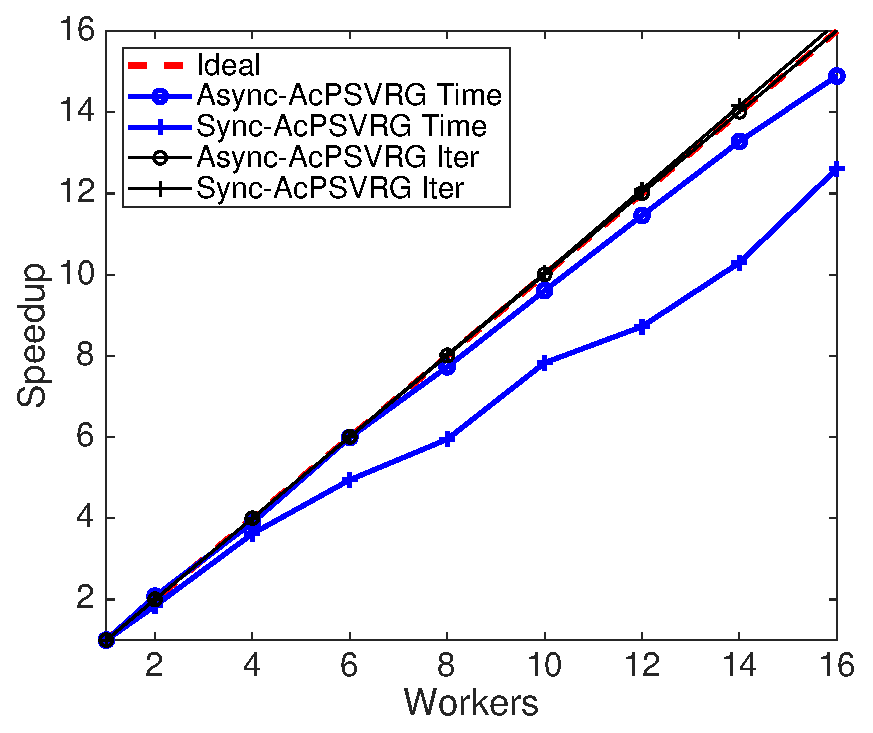
\includegraphics[width=0.33\linewidth]{Figures/ijcnn_speedup_FSVRG.eps}}%
\caption{Scalability analysis of Sync-AcPSVRG and Async-AcPSVRG with iteration and time speedup. }
\label{fig:FSVRG_speedup}
\end{figure}


\begin{figure}
\subfigure[covtype]{
\centering
\includegraphics[width=0.32\linewidth]{Figures/covtype_loss_comparison.eps}}%
\subfigure[w8a]{
\centering
\includegraphics[width=0.32\linewidth]{Figures/w8a_loss_comparison.eps}}%
\subfigure[ijcnn]{
\centering
\includegraphics[width=0.32\linewidth]{Figures/ijcnn_loss_comparison.eps}}

\subfigure[covtype]{
\centering
\includegraphics[width=0.32\linewidth]{Figures/covtype_obj_dev_comparison.eps}}%
\subfigure[w8a]{
\centering
\includegraphics[width=0.32\linewidth]{Figures/w8a_obj_dev_comparison.eps}}%
\subfigure[ijcnn]{
\centering
\includegraphics[width=0.32\linewidth]{Figures/ijcnn_obj_dev_comparison.eps}}

\caption{Comparison of convergence of asynchronous SVRG, ProxASAGA, Katyusha, and Async-AcPSVRG for logistic regression problems. Training loss (top) and residual (down). }
\label{fig:algo_comp}
\end{figure}

\[
 \text{iteration speedup} = \frac{\text{iteration cost for server with 1 worker}}{\text{iteration cost for server with n workers}} \]
\vspace{0.5 pt}
\[
  \text{time speedup} = \frac{\text{time cost for server with 1 worker}}{\text{time cost for server with n workers}}
\]








